% \pagebreak[4]
% \hspace*{1cm}
% \pagebreak[4]
% \hspace*{1cm}
% \pagebreak[4]
\chapter{Literature Review}
%\ifpdf
%    \graphicspath{{Literature/LiteratureFigs/PNG/}{Literature/LiteratureFigs/PDF/}{Literature/LiteratureFigs/}}
%\else
%    \graphicspath{{Literature/LiteratureFigs/EPS/}{Literature/LiteratureFigs/}}
%\fi




Paul Ehrlich famous quote is, ``To err is human, but to really foul things up you need a computer". Since the programmers are ordinary human beings, it is most obvious that some errors remain in the software after its completion. Errors are not tolerated as they can cause great loss. According to the National Institute of Standard and Technology 2002, 10 report, software errors cost an estimated \$59.5 billion loss to US economy annually. The destruction of the Mariner 1 rocket (1962) that cost \$18.5 million was due to a simple formula coded incorrectly by a programmer. The Hartford Coliseum Collapse (1978) costing \$70 million, Wall Street crash (1987) costing \$500 billion, Failing of long division by Pentium (1993) costing \$475 million, Ariane 5 Rocket disaster costing \$500 million and many others are caused by minor errors in the software. To achieve high quality, the software has to satisfy rigorous stages of testing. The more complex and critical the software, the higher the requirements for software testing and the larger the damage caused if the bug remains in the software. 

\section{Software Testing}
In the IEEE standard glossary of software engineering terminology \cite{american1984}, testing is defined as the process of exercising or evaluating a system or system component by manual or automated means to verify that it satisfies specified requirements and actual results. A successful test is one that finds a fault \cite{Myers2004}, where faults are defined as the errors made by the people during software development \cite{american1984}.

Being an integral part of Software Development Life Cycle (SDLC), the testing process is started from requirements phase since this is the starting point of all the software activities and continue throughout the life of the software. In traditional testing when testers finds a fault in the given SuT, the software is given back to the developers for removing the fault and after its rectification the software is handed back to the testers for retesting. It is important to understand the fact that ``program testing can be used to show the presence of bugs, but never to show the absence of bugs" \cite{Dijkstra1972}. Which means SUT that passes all the tests without giving a single error is not guaranteed to contain no error. The testing process increase however the reliability and confidence of the users in the tested product.


\begin{table}[ht]
%\scriptsize
\caption{Parts of Software Testing \cite{adrion1982validation}, \cite{chilenski1994applicability}, \cite{gaudel2010software}, \cite{richardson1992specification}, \cite{tracey1998automated}} % title of Table
\smallskip
\centering % used for centering table
\begin{tabular}{| l | l | l | l | } % centered columns (4 columns)
\hline

Levels 		&Purpose		 						& Perspective		& Execution 	\\
\hline
1. Unit		&1. Functionality						& 1. White Box		& 1. Static 	\\
2. Integration	&2. Structural							& 2. Black Box		& 2. Dynamic	\\
3. System		&3. Robustness						& 3. Grey Box		&			\\
			&4. Stress								&				&			\\
			&5. Compatibility						&				&			\\
			&6. Performance						&				&			\\



\hline %inserts single line
\end{tabular}
\bigskip
\{table:addvalues} % is used to refer this table in the text
\end{table}


\subsection{Software Testing Levels}
Unit testing, integration testing and system testing \cite{chilenski1994applicability} are the three main levels of software testing defined in the literature. Unit testing evaluate a small piece of software code called units for faults. These units are combined together to form components and integration testing ensure that the integration points are working properly. Finally the components are combined to form a system and before production system testing is performed to make sure that it works as expected. 


\subsection{Software Testing Purpose}
The primary purpose of software testing is identification of faults in the given SuT so that they can be corrected to achieve high quality. Ideally, maximum number of faults can be identified if software is tested exhaustively i.e. testing SuT against all possible combinations of input data, and comparing the obtained results to the expected results for assessment. However, exhaustive testing is not always possible in most of the test scenarios because of limited resources and infinite number of input values that a software can take. Therefore, the purpose of testing is generally directed to achieve confidence in a specific aspect of a SuT. For example, functionality testing is performed to check if one or more functions of a system are working correct or not. Structural testing analyse the code structure to generate test cases in order to evaluate paths of execution and identification of unreachable or dead code.  In robustness testing the software behaviour is observed in the case when it receive input that is outside of its expected input range.  Stress and performance testing aim to test the response of software under high load and its ability to process different nature of tasks \cite{cohen2005robustness}. Finally, compatibility testing is performed to see the interaction of software with underlying operating system or hardware.
 %As proper planning is the key to success for many projects this is often also true with software testing. A software test plan is a well defined document that defines the goal, scope, method, resources and time schedule of the testing.
%A software testing technique in which a software is tested with all possible combination of inputs. This technique can prove conclusively that the software meet its specification however exhaustive testing is seldom feasible because of the large input domain or too many paths in a software code. 

\subsection{Software Testing Perspective}
Testing activities can be split up into blackbox and whitebox testing on the basis of perspective taken. In blackbox or functional testing the testers dont need to know about internal code structure of the SuT. Test cases are derived from the specifications and test passes if the output is according to expected output. Internal code structure of the SuT is not taken into any consideration \cite{beizer1995black}. Whereas in whitebox or structural testing testers must know about the complete structure of the software and can modify it, if required. Test cases are derived from the code structure and test passes only if the results are correct and the expected code is followed during test execution \cite{ostrand2002white}.

%\subsubsection{Grey-Box Testing}
%Grey-Box testing is the combination of both black-box/functionality and white-box/structural testing. The tester knows about both the functionality and the internal structure of the SUT. Some of the test cases are based on the functionality and some of the test cases are based on the structure. Emphasis of grey-box testing is both on code coverage as well as functionality \cite{Savenkov2008}.

%\subsection{Software Testing Workflow}
%There are many software techniques like unit testing, integration testing, random testing, regression testing, system testing, acceptance testing, performance testing, load testing, stress testing, alpha testing, beta test etc. All testing techniques belong to black-box, white-box or grey-box approach. Each testing technique has its own strength and weaknesses but the technique in focus here is Random Testing.


%\begin{figure}[h]
%\begin{center}
%	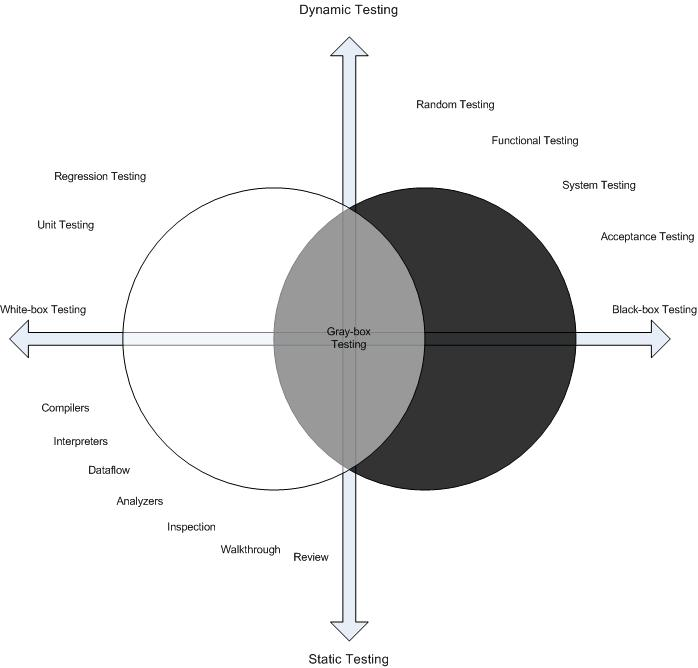
\includegraphics[width=16cm, height=12cm ]{Literature/Drawing34.jpg}
%	\caption{Software Testing Workflow}
%\end{center}  
%\end{figure}


%We have explained software testing graphically with the help of plotting venn diagram on two dimensional axis. The positive x axis represent black-box while negative x axis represent white-box testing. Grey-box testing in the middle is represented by the overlapping of black-box and white-box testing. Similarly on positive y axis we have dynamic testing and on negative y axis we have static testing.
%Now if a test is black box and dynamic then the test will fall in 0 to 90 degree on the diagram and if the test is black-box and static then it will fall in 270 to 360 degree. On the other hand if the test is white-box and dynamic then it will fall in 90 to 180 degree and if the test is white-box and static then it will fall in 180 to 270 degrees.




\subsection{Software Testing Execution}
Test activities can be organised into static and dynamic testing on the basis test cases execution. In static testing test cases analysed statically checked for errors without any execution. All high quality softwares are accompanied by documentation in addition to software code. These include requirements, design, technical, end-user and marketing documentation. Reviews, walkthroughs or inspections are most commonly used techniques for static testing. In dynamic testing the software code is executed and input is converted into output through processing. Results are analysed against expected results to find any error in the software. Unit testing, integration testing, system testing, and acceptance testing are most commonly used as dynamic testing methods \cite{fairley1978tutorial}

%Dynamic testing can be manual or automated. In manual testing the programmer develops the test cases which are executed by the developed software to find any error in processing or output. Similarly in automated testing the software or components of the software is given as input to testing software that automatically generates test cases and executes the SUT against them to find any errors. Manual testing typically consumes more time and resources than automated testing.



\subsection{Manual Testing}
 A software testing technique to find faults in a class or group of related classes, such that the tester must write the code by hand to create test cases and test oracle \cite{Ciupa2008}. While manual testing is effective in some cases, in general, it is a laborious, time consuming, error-prone \cite{tretmans1999}. It further requires testers to have appropriate skills, experience and in depth knowledge of the under test software in order to evaluate it from different perspectives.
 
\subsection{Automated Testing}
A software testing technique to find faults in a class or group of related classes, such that the test cases and test oracle is generated automatically by a testing tool \cite{Leitner2007}. The tools can automate part of a test i.e. generation of test cases, execution of test cases and evaluation of results or the whole test process. The use of automated testing made it possible to test large volumes of code that would be otherwise impossible \cite{ramamoorthy1975}.

%\section{Automated Random Testing}
%\subsection{Test Data Generation}
%\subsection{Test Execution}
\subsection{Test Oracle}
Test oracles set the acceptable behaviour for test executions \cite{richardson1992specification}. All softwares testing techniques depend on the availability of a test oracle \cite{baresi2001test}. Designing test oracles for simple softwares may be straight forward, however, for relatively complex softwares it can be very cumbersome to decide whether a program execution returns a correct or incorrect result \cite{gaudel2010software}. Different testing techniques tackle the oracle problem in various ways but some of the common issues include:
\begin{enumerate}
\item It is assumed that execution results are observable, so that they can be evaluated against the test oracle or the oracles are defined on the basis of these results.
\item An ideal test oracle would satisfy desirable properties of program specifications \cite{baresi2001test}.
\item There is not a single oracle generation technique that satisfies all purposes. Weyuker \cite{weyuker1982testing} argued that truly general test oracles are often unobtainable.
\end{enumerate}
%\subsection{Test Report}

\subsubsection{Random Testing}
Random testing is a dynamic and black-box testing technique in which the software is tested with non-correlating or unpredictable test data from the specified input domain \cite{Chan2002}. The input domain is a set of all possible inputs to the software under test. According to Richard H. \cite{hamlet1994}, to conduct random testing, an input domain is defined, then test points are randomly taken from the whole input domain through a random number/test case generator. The program under test is executed on these points and the results obtained are compared to the program specifications. The test fails if any input leads to incorrect results or otherwise it is successful. 

\begin{figure}[h]
	\centering
	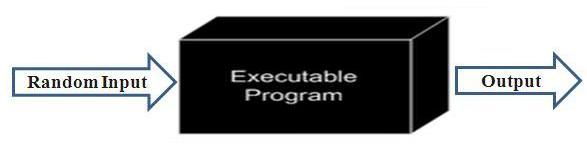
\includegraphics[scale=0.5]{Literature/figure1.jpg}
	\caption{Random Testing}
\end{figure}

It is quick and cheap to generate random test data as it don't require too much intellectual and computational efforts \cite{Ciupa2009}. This capability makes it an ideal choice for implementation in automated testing tools \cite{Ciupa2008a}. In addition, no human intervention in data generation/selection makes it one of the most unbiased testing technique. 

Generating test cases with out using any background information makes it highly susceptible to criticism. Myers \cite{Myers1979} intuitively mentioned random testing as one of the least effective testing technique. It is also criticised for generating many sets of tests that lead to the same state of the software. Furthermore, random testing can generate test inputs that violates requirements of the given SUT making it less effective \cite{sen2007effective}, \cite{pacheco2009directed}. 

Myers statement was not based on any experimental evidence and later on the experiments performed in \cite{hamlet1994}, \cite{Ciupa2008}, \cite{leitner2007efficient} and \cite{Duran1981} confirmed that random testing is as effective as any other systematic testing technique. The experiments in \cite{Duran1981} found that random testing can find subtle faults in a given SUT if run for large number of test cases. They argued that the simplicity and cost effectiveness of random testing can make it feasible to run large number of test cases as opposed to systematic testing which requires considerable time and resources for test case generation and execution. The empirical comparison \cite{hamlet1990} also prove that random testing and partition testing are equally effective. Furthermore the study conducted by Ntafos \cite{ntafos1998random} conclude the effectiveness of random testing over proportional partition testing.



\section{Variations in Random Testing}
Different researchers tried various strategies to improve the performance of random testing. In order to better understand the topic we have studied each strategy in detail.

\subsection{Adaptive Random Testing}
Adaptive random testing (ART) \cite{Chen2008} is based on the existence of failure patterns across the input domain detected by Chan et al \cite{Chan1996}. They observed that failure inducing inputs in the whole input domain form certain geometrical patterns. They divided these patterns into point, block and strip fault patterns. Each one is described below.

\begin{figure}[h]
	\centering
	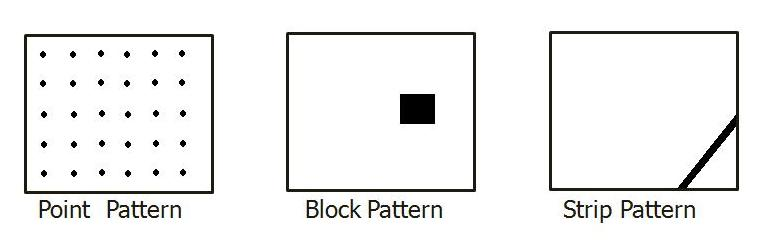
\includegraphics[scale=0.5]{Literature/pointblockstrip}
	\caption{Patterns of failure causing inputs}
	\label{fig:patterns}
\end{figure}

In the figure \ref{fig:patterns} the square box indicates the whole input domain. The white space shows legitimate or faultless values while the black colour points, block and strip inside each box indicate the point, block and strip fault patterns in the input domain.

\begin{enumerate}
\item Point pattern: In the point pattern failure inducing inputs are scattered across the input domain in the form of stand-alone points. Example of point pattern is the division by zero in a statement total = num1/num2; where num1, num2 and total are variables of type integer. 
\item Block pattern: In the block pattern multiple failure inducing inputs lies in a close vicinity to form a block in the input domain. Example of block pattern is failure caused by a statement if ( (num \textgreater 10) \&\& (num \textless 20) ). Here 11 to 19 is a block of faults.
\item Strip pattern: In the strip pattern the failure inducing inputs form a strip across the input domain. Example of strip pattern is failure caused by a statement num1 + num2 = 20. Here multiple values of num1 and num2 can lead to the fault value 20.
\end{enumerate}

The authors argued that ordinary random testing may generate test inputs lurking too close or too far from the fault inducing input and thus failing to discover it. To generate more fault targeted test inputs they suggested ART. ART is a modified version of ordinary random testing where test values are selected at random like before but evenly spread across the input domain. To achieve an even distribution of test cases across the input domain they used two sets. The executed set having the test cases that have been executed by the system and the candidate set that contain the random selected test cases from the bounded input domain as candidates for execution. Initially both the sets are kept empty. The first test case is selected at random from the candidate set and stored in executed set after execution, the second test case is then selected from the candidate set based on the criteria that it is far away from the last executed test case. Thus the whole input domain can be tested and their are more chances of generating test input from inside of the existing geometrical patterns. 

In the experiments they used number of test cases required to detect first failure (F-measure) as a performance matrix instead of the traditional matrix i.e. probability of detecting at least one failure (P-measure) and expected number of failures detected (E-measure). Results of the experiments performed on published programs using ART showed up to 50\% increase in the performance of than ordinary random testing. Results showed significant improvement, however, the issues of increase overhead, spreading test cases across the input domain for complex objects and efficient ways of selecting candidate test cases still exist. Chen et al evolve their work on ART to address some of these issues in \cite{chen2009enhanced} and \cite{Chen2005}. 

\subsection{Mirror Adaptive Random Testing}
As discussed in the above section ART provide better results, however the increase in overhead due to extra computation to achieve even spread of test inputs makes it less cost effective. Mirror Adaptive Random Testing (MART) \cite{Chen2003} is an innovative approach that uses mirror partitioning technique to reduce the overhead of ART by decreasing the extra computation involved in ART.

\begin{figure}[h]
\begin{center}
	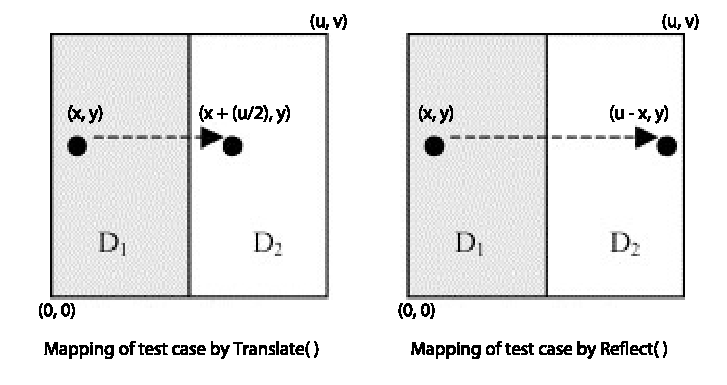
\includegraphics[width=13cm, height=6cm ]{Literature/mart2.pdf}
	\caption{Mirror Adaptive Random Testing \cite{Chen2003}}
\label{fig:mirrorART}
\end{center}  
\end{figure}

In this technique, the input domain of the program under test is divided into n disjoint subdomains of equal size and shape. One of the subdomain is called source subdomain while all the others are termed as mirror subdomains. ART is then applied only to the source subdomain to select the test cases and from all other subdomains test cases are selected by using mirror function. In MART \{(0, 0), (u, v)\} are used to represent the whole input domain where (0, 0) are the leftmost and (u, v) are the rightmost top corner of the two dimensional rectangle. On splitting it into two subdomains we get \{(0, 0), (u/2, v)\} as source subdomain and \{(u/2, 0), (u, v)\} as mirror subdomain. Let suppose we get x and y test cases by applying ART to source subdomain, now we can linearly translate these test cases to achieve the mirrored effect, i.e. (x + (u/2), y) as shown in the figure \ref{fig:mirrorART}. Experimental results showed that the performance of MART is equal to ART with MART using only one quarter of the calculations of that of ART.    


\subsection{Restricted Random Testing}
Restricted Random Testing (RRT) \cite{chan2003normalized} is another approach, with small overhead in contrast to ART, to spread the the test cases more evenly across the input domain. RRT achieves this by creating a circular exclusion zone around the executed test case. A candidate is randomly selected from the input domain for the next test case. Before execution the candidate is checked and is discarded if it lies inside the exclusion zone. This process repeats until a candidate laying outside the exclusion zone is selected. This ensures that the test case to be executed is well apart from the last one. The radius of exclusion zone is constant around each test case and the area of each zone decreases with successive cases.

\begin{figure}[h]
	\centering
	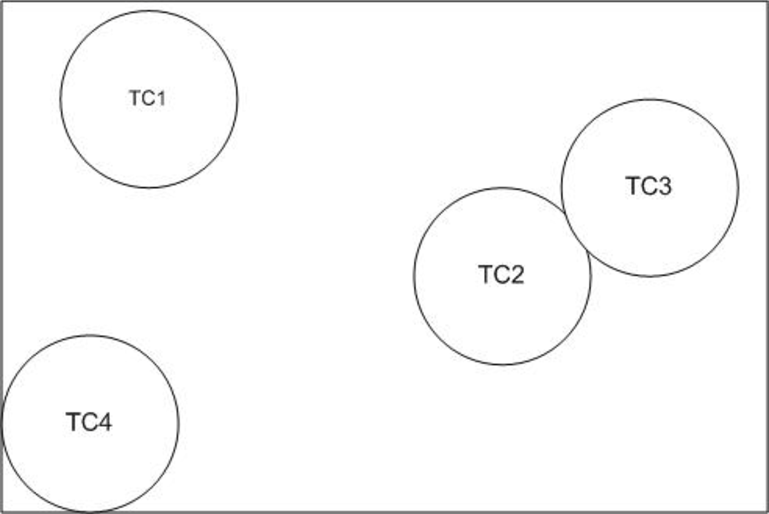
\includegraphics[width= 6cm, height = 5cm]{Literature/RRT.pdf}
	\caption{Input domain with exclusion zone around the selected test case}
\end{figure}

To find the effectiveness of RRT, the authors compared it with ART and RT on 7 out of the 12 programs evaluated by ART and MART. The experimental results showed that the performance of RRT increases with the increase in the size of the exclusion zone and reaches to maximum when the exclusion zone is raised to largest possible size. Normalized Restricted Random Testing \cite{chan2003normalized} is an improvement over RRT by allowing the testers to have better information about the target exclusion rate (R) of RRT. They further found that RRT is up to 55\% more effective than ordinary random testing in terms of F-measure (Where F-measure is the total number of test cases required to find the first failure).



\subsection{Directed Automated Random Testing}
Directed Automated Random Testing (DART) is a random testing technique proposed by Godefroid et al., \cite{Godefroid2005}. Its main purpose was to overcome the cost and difficulty of manual testing while keeping its quality intact. It automate the whole testing process including generation of unit tests, test drivers/harness and assertions for functional correctness. The main functions of DART can be divided into three parts;
\begin{enumerate}
\item Automated Interface Extraction: DART automatically identifies external interfaces of a given SUT. These interfaces include external variables, external functions and the user-specified main function which initialises the program execution.
\item Automatic Test Driver/Harness: After identification of all the external interfaces of a given SUT, DART generate test drivers/harness to run the test cases. All the test cases are randomly generated according to the underlying environment.
\item Dynamic Analysis of execution: The DART instrument the given SUT at the start of the process in order to track its behaviour dynamically at run time. The results obtained are analysed in real time to systematically direct the test case execution along alternative path for maximum code coverage.
\end{enumerate}

Directed Automated Random Testing algorithm is implemented in DART tool. It is a completely automatic tool and all it needs is a test program as input. After the external interfaces are extracted it then use the pre-conditions and post-conditions of the program under test to validate the test inputs. For languages that do not support contracts inside the code (like C), they used public methods or interfaces to mimic the scenario  ---------------------------- to be continued.

\subsection{Quasi Random Testing}
Quasi-random testing (QRT) \cite{Chen2005} is a testing technique that takes advantage of failure region contiguity by distributing test cases evenly similar to ART but with decreased computation. Chan et al after the analysis of faults in various experiments found that the fault patterns across the input domain are continuous. To achieve even spreading of test cases, QRT uses a class with a formula, that forms an s-dimensional cube in s-dimensional input domain and generate sequence of numbers that have small discrepancy and low dispersion. These sequence of numbers are then used to generate random test cases that are permuted to make them less clustered and more even than RT. An empirical study was conducted to compare the effectiveness of QRT with ART and RT. The 12 numerical programs picked for experiments were the same used to evaluate ART.The empirical results of the experiments showed that in 9 out of 12 programs QRT on average finds a fault quickly than ART and RT while in the remaining three programs the improvement is insignificant.
%\subsection{Monti Carlo Random Testing}

%\subsection{Good Random Testing}

\subsection{Feedback-directed Random Testing}
Feedback-directed Random Testing (FDRT) \cite{Pacheco2007} is a technique that generate unit test suite at random for object oriented programs. As the name implies FDRT uses the feedback received from the execution of first batch of randomly selected unit test suite to generate next batch of more directed unit test suite. In this approach redundant and illegal unit tests are eliminated incrementally from the test suite with the help of filtration and application of contracts. For example unit test that produce IllegalArgumentException on execution is discarded, because, randomly selected argument used in this test was not according to the type of argument the method required.

\subsubsection{Randoop: Feedback-directed Random Testing}
The FDRT technique is implemented in RANDOOP tool \cite{Pacheco2007b}. RANdom tester for Object Oriented Programs (RANDOOP) is a fully automatic tool, capable of testing Java classes and .Net binaries. RANDOOP takes as input a set of classes (java or .Net executables), contracts, filters and the time limit after which the testing process stops. Its output is a suite of JUnit and NUnit for Java and .Net programs respectively. Each unit test in a test suite is a sequence of method calls (hereafter referred as sequence). RANDOOP build the sequence incrementally by randomly selecting a public method from the class under test and arguments for these methods are selected from the predefined pool in case of primitive types and a sequence or null value in case of reference type. RANDOOP maintains two sets called ErrorSeqs and NonErrorSeqs to record the feedback. It extends ErrorSeqs set in case of contract or filter violation and NonErrorSeqs set if no violation is recorded in the feedback. The use of this dynamic feedback evaluation at runtime bring an object to very complex and interesting state. On test completion it produce ErrorSeqs and NonErrorSeqs as JUnit/NUnit test suite. To find the effectiveness of the strategy, in terms of coverage and number of faults discovered, the authors compared RANDOOP implementing FDRT with random testing of JCrasher and JavaPathFinder \cite{visser2004test}. In the experiments 14 libraries of both Java and .Net were evaluated.  The results showed that RANDOOP achieved more coverage than JCrasher in behavioural, branch coverage and faults detection. It can achieve on par coverage with systematic approaches like JavaPathFinder. RANDOOP also has an edge over model checking for its ability to easily search large input domains.
%\subsection{Adaptive Random Testing for Object-Oriented}



\subsection{Object Distance and its application}
To improve the performance of random testing the emphasis of ART was on the distance between the test cases. But this distance was defined only for primitive data types like integers and other elementary input. Ciupa et al defined the parameters that can be used to calculate distance between the composite programmer-defined types so that ART can be applicable to testing of todays object-oriented programs \cite{Ciupa2006}. Two objects have more distance between them if they have more dissimilar properties.
The parameters to specify the distance between the objects are dynamic types, values of its primitive and reference fields. Strings are treated as a directly usable values and Levenshtein distance \cite{Levenshtein1966} which is also known as edit distance is used as a distance criteria between the two strings.
To implement object distance first all the distances of the objects are measured. Then two sets candidate- objects containing the all the objects ready to be run by the system and the used-objects set which is initially empty. First object is selected randomly from the candidate-object set and is moved to used- object set when executed by the system. Now the second object selected from the candidate set for execution is the one with the biggest distance from the last executed object present in the used-object set. This process is continue until the bug is found or the objects in the candidate-object set are finished.

\subsubsection{ARTOO Tool}
After the criteria to calculate the distance between the objects is defined \cite{Ciupa2006}, the same team implemented that model and performed several experiments to evaluate the proposed model. Adaptive Random Testing for Object Oriented (ARTOO) is a testing strategy, based on object distance, implemented in AutoTest tool [16].
ARTOO was implemented as a plug-in strategy in AutoTest. It only deals with creating and selecting inputs and all other functionality of the AutoTest was the same. Since ARTOO is based on object distance therefore the method for test input selection is to pick that object from the candidate set (A pool of objects that is a potential candidate to be executed by the system) which has the highest average distance in comparison to the objects already executed.
In the experiments classes from EiffelBase library [17] were used. To evaluate ARTOO the same tests were also applied to directed random strategy (RAND). The outcome of the experiments showed that ARTOO finds the first bug with fewer test cases than RAND. The computation to select test case in ARTOO is more than RAND and therefore ARTOO takes more time to generate a test input. The experiments also found few of the bug found by ARTOO were not pointed out by RAND furthermore ARTOO is less sensitive to the variation of seed value than RAND.

\subsubsection{Experimental Assessment of RT for Object-Oriented Software}
In this research the effect of various parameters involved in random testing and its effect on efficiency is evaluated by performing various experiments on Industrial-grade code base.
Large scale clusters of computers were used for 1500 hours of CPU time which resulted in 1875 test sessions for 8 classes under test. \cite{Ciupa2007} The finding of the experiments are
1. Version of random testing algorithm that is efficient for smaller testing timeout is equally efficient for higher testing timeouts.
2. The value of seed for random testing algorithm plays a vital role in finding the number of bugs in specific time.
3. Most of the bugs are found in the first few minutes of the testing sessions.


%\section{Automated Random Testing Tools}

\subsection{JCrasher}

JCrasher is first of the three automatic testing tools developed by Csallner C. and Smaragadakis Y. \cite{Pacheco2007b}. As the name suggests JCrasher tries to crash the Java program with random input and any exceptions thrown during the process are recorded. All exceptions are then compared to the list of acceptable exception, which are defined in advance as heuristics, any undefined/undeclared runtime exceptions are considered errors. Since programs interact with the world through its public methods and they are also exposed to different kind of inputs, therefore, JCrasher tests only these methods with random inputs. 

\begin{figure}[h]
	\centering
	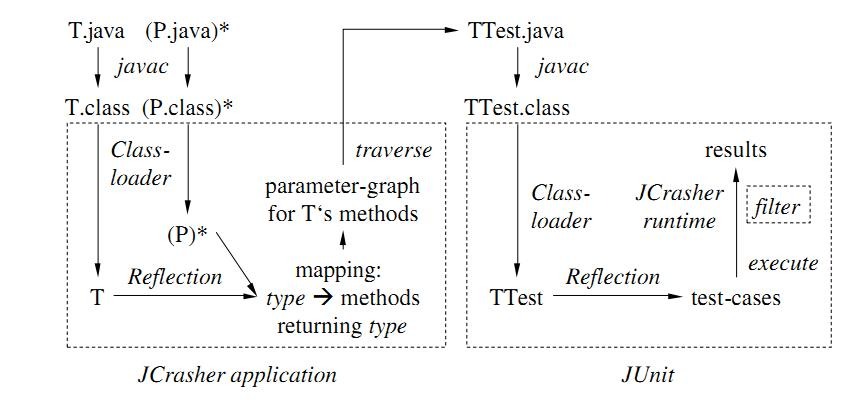
\includegraphics[width=15cm, height=7cm]{Literature/jcrasher.png}
	\caption{Process of robustness testing of java program with JCrasher \cite{Pacheco2007b}}
	\label{fig:jcrasher}
\end{figure}

Figure \ref{fig:jcrasher} illustrate the working of JCrasher by testing a java program namely T.java. The source file is first compiled using javac and the obtained byte code is passed into JCrasher. The JCrasher using Java reflection \cite{chan1999java}  analyse all the methods declared by class T and by their transitive parameter types P to generate the most appropriate test data set. The test data set is written to a file TTest.java that is compiled and executed by JUnit. All the exceptions produced during test case executions are collected and compared with robustness heuristic to check for violation. Any violated test case is reported as error.\\

JCrasher is a pioneer to perform fully automatic testing from test case generation, execution, filtration to reporting the results. One of its novelty  is that it generates test case as JUnit files that can be easily read and can be used for regression testing. Another important feature of JCrasher is to execute each new test on a ``clean slate" ensuring that the changes made by the previous tests do not affect the new test.  

% check parameter space or parameter graph in the figure???


\subsection{Jartege}
Jartege (\uline{Ja}wa \uline{r}andom \uline{te}st \uline{ge}nerator) \cite{Oriat2004} is an automated testing tool that randomly generates unit tests for Java classes with contracts specified in Java Modelling Language (JML). The contracts include methods pre- and post-conditions and class invariants. Initially Jartege uses the contracts to eliminate irrelevant test cases and later on the same contracts serve as test oracle to differentiate between errors and false positives. Jartege uses simple random testing to test classes and generate test cases, however, it facilitate to parameterise its random aspect in order to prioritise testing specific part of the class or to get interesting sequences of calls. These includes: 
\begin{itemize}
\item To define the operational profile of the classes i.e. the likely use of the class under test by other classes.  
\item To define the weight of each class and method under test and give test priority to the one's with highest weight and skip those with null weight.
\item To control the creation of newly created objects with creation probability functions. Low probability means creation of fewer objects and more reusability for different operations while high probability means numerous new objects with less reusability.
\end{itemize}

\noindent The Jartege technique evaluate class by entry pre-condition and internal pre-condition. Entry pre-conditions are the contracts which must be met by the generated test data to test the method while internal pre-conditions are the ones which are inside the methods and their violation are considered error either in method or in the specification. The benefits of Jartege is that it checks for errors in both program and specifications and the Junit tests produced by Jartege can be used later as regression tests. Its minor short coming is that the SUT JML specifications must exist or may be written manually in order to be tested by Jartege.

\subsection{Eclat}
Eclat \cite{Pacheco2005} testing tool automatically generates and classify unit tests for Java classes. The process can be divided into three main components. In the first component, it selects small subset of test inputs, likely to reveal faults in the given SUT, from a large set of test inputs. The tool takes a software and a set of test cases for which the software runs properly. It then creates an operational model based on the correct software operations and apply the test data to it. As a result any inputs whose operational pattern of execution differs from the operational model are (1) likely to reveal fault in the given SUT, (2) Likely to produce normal operations despite violating the model, (3) illegal input that the program is not required to handle. In the second component, reducer function is used to discard any redundant input, leaving only one input per operational pattern.The third and final component facilitate automated testing by converting the acquired test inputs into test cases and creation of oracle to determine whether the test succeeds or fail. \\
\indent To measure the effectiveness, the researchers tested 9 programs on both Eclat and JCrasher \cite{Pacheco2007b}.  The experimental results revealed that Eclat outperformed JCrasher. On average, Eclat selected 5.0 inputs per run, and 30\% of those revealed a fault. While JCrasher selected 1.13 inputs per run, and 0.92\% of those revealed a fault. The short coming of Eclat is its dependence on the initial pool of correct test cases which is usually written manually and existence of any errors in it can propagate and affect the whole testing process.    
\subsection{JTest}
Parasoft Jtest is a commercial tool that automatically generates and execute unit tests. It can be easily integrated to Java IDEs like Eclipse where it provide two main functionalities, i.e. Static Analysis, Unit testing and code coverage. [25]
In static analysis Jtest takes a complete project or set of classes as input and compares it with a list of built-in rules. The statement violating any of these rules is an error. It also suggests probable fixes for the detected fault.
For unit testing it takes a class as an input and processes a number of scenarios against it to generate and execute unit tests. Once unit tests are executed they become the part of regression test for future reference.
Jtest also shows the code coverage of the program by colour coding the statements that are not executed by the unit tests.

\subsection{QuickCheck}
QuickCheck \cite{Claessen2000} is a light weight random testing tool that is developed specifically for testing of Haskell programs \cite{Hudak2007}. Haskell is a functional programming language where programs are evaluated using expressions rather than statements as in case of imperative programming. Therefore in this process the tester defines certain expressions for the functions that must hold for a large number of test cases to be correct. These test cases are generated automatically through generator function which can be set by the tester to generate random test cases or according to specific criteria. After processing all the generated test cases any test case that causes the expression to become false is considered faults.

\subsection{AgitarOne}
AgitarOne is a commercial tool that automatically generates unit tests. It has a Junit Generator engine that can create 25,000 lines or more of Junit per hour [29]. It can be easily integrated into famous IDE like Eclipse. It takes as input, classes under test, time and optionally any knowledge or test cases that has a positive influence on the performance of the testing process. The generated Junit tests can be run from the same IDE and can also be used for later regression testing. The GUI interface is called a dashboard which provides in depth knowledge of the tests conducted, failures detected, alerts and the archieves of the tests conducted earlier. It also shows the coverage obtained after executing the Junits against the code under test.

\subsection{Autotost}
Based on Formal Automated testing AutoTest is a tool used for testing of Eiffel programs \cite{Ciupa2007}. The Eiffel language use the concept of contracts (pre-conditions, postconditions and class invariants). Input can be a single class, method or a set of classes which is then processed by AutoTest to generate test cases. It generates both primitive and object type test cases. All the generated test cases are kept in a pool and then randomly a test case is selected from it for execution. A user can set the features of the AutoTest options include: Number of test cases to generate, whether to monitor pre or post condition, order of testing and the initial values of the primitives variables.

\subsection{TestEra}
TestEra \cite{Khurshid2004} is a novel framework for testing Java applications. All the tests are produced and executed in an automated fashion. Tests are conducted on the basis of the method specifications \cite{Chang1999}. TestEra takes methods specifications, integer value as a limit to the generated test cases and the method under test. It uses pre-conditions of a method from specifications to automatically generate test cases up to the specified limit. These test cases are then executed on the method and the result is compared against the postconditions (oracle) of that method. Any test case that fails to satisfy postcondition is considered as a fault. The complete error log is displayed in the Graphical User Inteface (GUI).

\subsection{Korat}
Korat \cite{Boyapati2002} is an automated testing tool for Java programs that generates and execute test cases for a method based on its formal specification. To generate test cases for a method Korat makes use of its pre-condition. It then executes the generated test cases against the method specifications. Korat uses JML for specifications. In order to generate test cases for a method Korat constructs new methods that return a Boolean value (Java Predicate) from its pre-conditions. When given these Java predicates Korat generates all non isomorphic input for which the return value of predicate is true. To check correctness of the method, Korat executes the test cases on that method and analyzes the output with the post conditions of the method (oracle). A fault in a method under test throws an exception to indicate the violation of the post-condition.

\subsection{YETI}
York Extensible Testing Infrastructure (YETI) is an automated tool for testing Java, JML and .NET assemblies \cite{Oriol2010c}. YETI execute the program under test with random generated but type-correct inputs and declare a fault if the response is an unexpected exception or a contract violation. YETI has been designed with an emphasis on extensibility. Its three main parts: the core infrastructure, strategies and language bindings are loosely coupled to easily accommodate new languages and strategies. To keep the process fully automated YETI uses two approaches for oracle (pass/fail judgement). If available, YETI uses code contracts as oracle if not it uses undeclared runtime exceptions of the underlying language as oracle. The test cases revealing errors are reproduced at the end of each test session for unit and regression testing. Other prominent features of YETI include its Graphical User Interface (GUI) for user friendliness and ability to distribute large testing tasks in cloud for parallel execution \cite{Oriol2010}. The following sections briefly describe internal working and execution of YETI tool. 

\subsection{Construction of Test Cases}
YETI construct test cases at random by creating objects of the class under test and randomly calling its methods with inputs according to its parameter's-space. Strategy section contains seven different strategies and inputs to the tested methods is defined by one of the selected strategy. To completely automate the data generation YETI   split input values into two types i.e. primitive data types and user defined classes. For Java primitive data types, which includes short, byte, char, int, float, double, long etc, YETI uses its own built-in random value generation library. However, in the case of user defined classes where objects data type is a user defined class YETI calls its constructor to generate object of that class at run time. It may be possible that the constructor require another object and in this case YETI will recursively calls the constructor of that object. This process is continued until the an object with blank constructor, constructor with only primitive types (type 1) or the set level of recursion is reached. 

\subsection{Commnad-line Options}
While YETI GUI launcher has been developed during this research study, to take maximum benefit of the available options one still need to launch YETI from CLI mode. These command-line options are case insensitive and can be provided as input to the tool in CLI mode. For example, to save processing power command line option -nologs can be used to bypass realtime logging. The following table describes few of the most common command-line options available in YETI.    

\begin{table}[h]
%\scriptsize
\caption{YETI command line options} % title of Table
\smallskip
\centering % used for centering table
\begin{tabular}{ll } % centered columns (4 columns)
\hline

Levels 					&Purpose 			\\
\hline
-java						&Test programs coded in Java	 	\\
-jml						&Test programs coded in JML			\\
-dotnet					&Test programs coded in .NET		\\
-ea						&To check code assertions \\
-nTests					&Specify number of tests after which the test stops	\\
-time						&Specify time in seconds or minutes after which the test stops\\
-testModules				&Specify one or more modules to test 	\\
-rawlogs					&Prints real time logs during test \\
-nologs					&Omit real time logs and print end result only\\
-yetiPath					&Specify path to the test modules\\ 
-gui						&Show test session in GUI\\
-DSSR					&Specify Dirt Spot Sweeping Random strategy for this session\\
-ADFD					&Specify Automated Discovery of Failure Domain strategy for this session\\
-random					&Specify random test strategy for this session\\
-randomPlus				&Specify random plus test strategy for this session\\
-randomPlusPeriodic		&Specify random plus periodic test strategy for this session\\
-nullProbability				&Specify probability of inserting null as input value\\
-newInstanceProability		&Specify probability of inserting new object as input value\\

\hline %inserts single line
\end{tabular}
\bigskip
\label{table:cliOptions} % is used to refer this table in the text
\end{table}


\subsection{YETI Execution}
YETI being developed in Java is highly portable and can easily run on any operating system with Java Virtual Machine (JVM). YETI can be executed from both command line and GUI. To build and execute YETI, it is necessary to specify the project and all the .jar library files particularly javassist.jar in the CLASSPATH or JVM would not be able to find and execute it. There are several options available as discussed in section xxx??? to accommodate specific needs but the typical command to invoke YETI is given in figure \ref{fig:XXX???}. In this particular command YETI tests java.lang.String and yeti.test.YetiTest modules, for details of other options please see section xxx????. 

\begin{figure}[h]
	\centering
	\frame{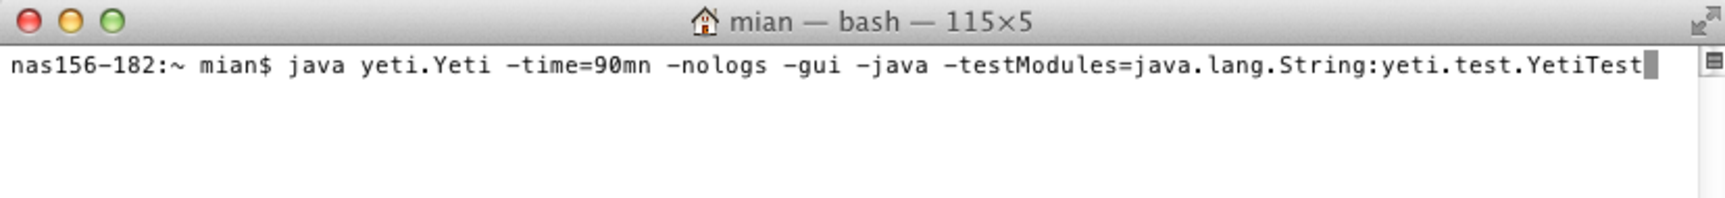
\includegraphics[width= 14cm, height = 1.8cm]{Literature/yetiCommandCLI.pdf}}
	\caption{Command to launch YETI from CLI}
\end{figure}

Alternately, runnable jar file by the name YetiLauncher is also available to launch YETI from GUI. However, till the writing of this thesis, the GUI version of YETI only supports the basic options of YETI. Figure xxx??? shows the equivalent of above command in GUI mode.

\begin{figure}[h]
	\centering
	\frame{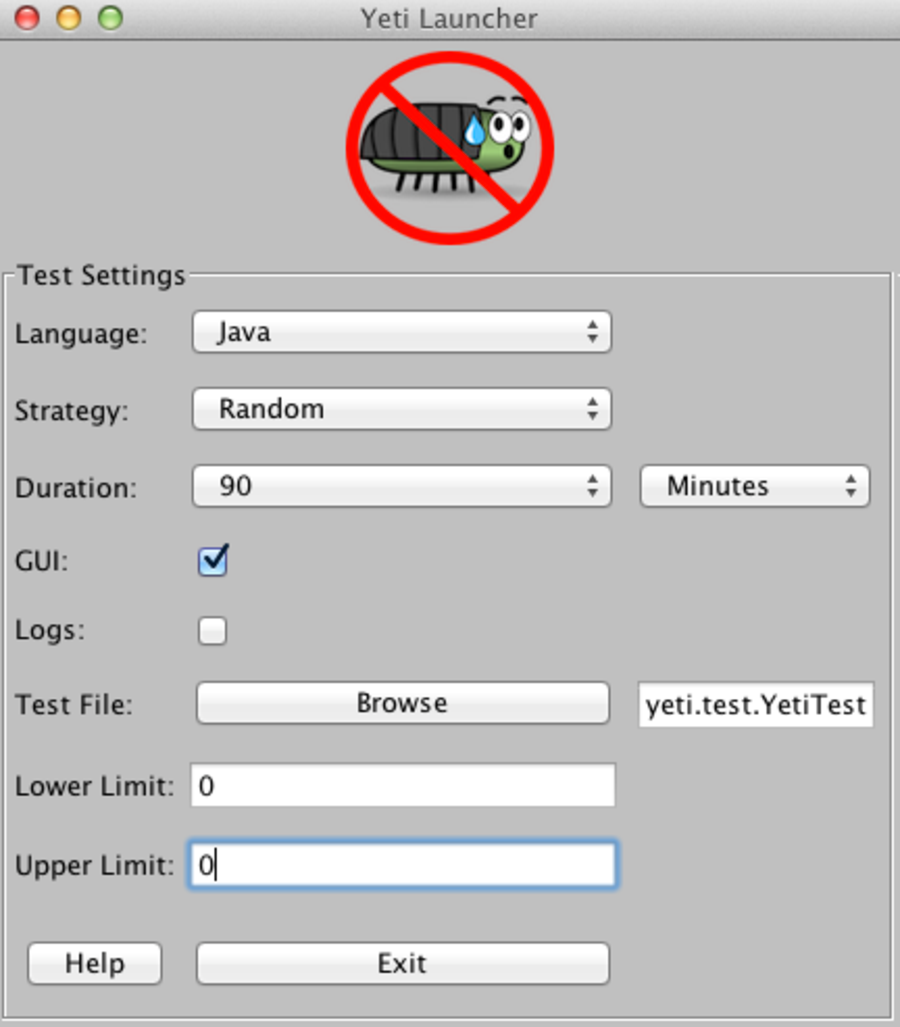
\includegraphics[width= 7cm, height = 8cm]{Literature/yetiCommandGUI.pdf}}
	\caption{Command to launch YETI from GUI}
\end{figure}


As a result of both the above commands YETI launch its own GUI window and start testing the assigned programs. 




\subsection{YETI Report}



\subsection{Tools for Automated Random Testing}
From the literature we can find a number of open source and commercial testing tools that automatically generate unit tests. Each tool utilize different generation technique but the one we are interested in is random technique. We present the most well known tools.

\begin{figure}[h]
	\centering
	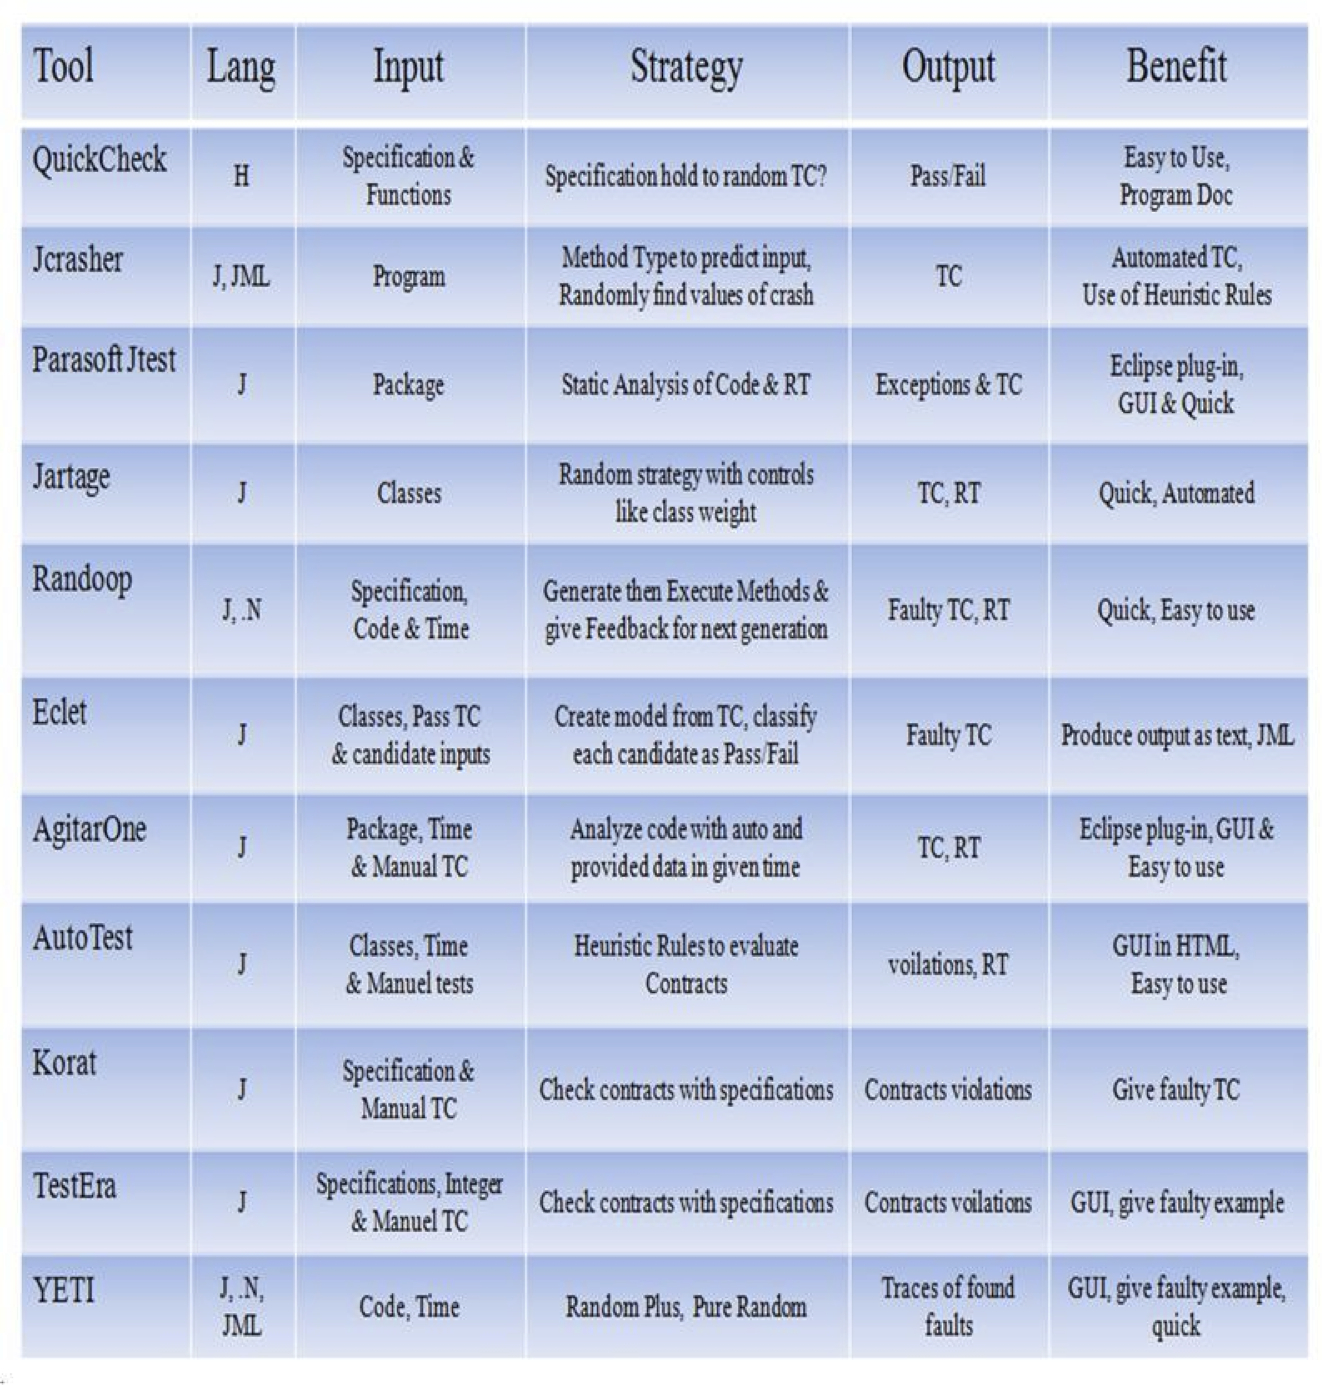
\includegraphics[scale=0.6]{Literature/tools}
	\caption{Summary of automated testing tools}
\end{figure}


\section{Conclusion}


% ------------------------------------------------------------------------


%%% Local Variables:
%%% mode: latex
%%% TeX-master: "../thesis"
%%% End:
